% Exact LaTeX recreation of the supplied Phase-1.pdf
% Compile with pdfLaTeX.

\documentclass[11pt,a4paper]{article}

\usepackage[a4paper,left=2.0cm,right=2.0cm,top=1.8cm,bottom=1.55cm]{geometry}
\usepackage[T1]{fontenc}
\usepackage{lmodern}
\usepackage{graphicx}
\usepackage{xcolor}
\usepackage{array}
\usepackage{tabularx}
\usepackage{ragged2e}
\usepackage{enumitem}
\usepackage{fancyhdr}
\usepackage{tikz}
\usepackage{setspace}
\usepackage{hyperref}

\definecolor{TitleBlue}{RGB}{61,103,154}

\setlength{\parindent}{0pt}
\setlength{\parskip}{0pt}
\renewcommand{\arraystretch}{1.0}

\newcommand{\blueheading}[1]{%
    {\sffamily\color{TitleBlue}\fontsize{15}{18}\selectfont #1}%
}

\newcommand{\bluebigheading}[1]{%
    {\sffamily\bfseries\color{TitleBlue}\fontsize{16}{19}\selectfont #1}%
}

\newcommand{\instruction}[1]{%
    {\itshape\fontsize{10.5}{12.5}\selectfont #1}%
}

\newcommand{\answerbox}[2][3.0cm]{%
    \vspace{2pt}
    \noindent
    \fbox{%
        \begin{minipage}[t][#1][t]{\dimexpr\textwidth-2\fboxsep-2\fboxrule\relax}
            \vspace{1mm}
            \itshape #2
        \end{minipage}
    }
}

% -------------------------------------------------
% HEADER / FOOTER
% -------------------------------------------------
\pagestyle{fancy}
\fancyhf{}
\renewcommand{\headrulewidth}{0pt}
\renewcommand{\footrulewidth}{0pt}

\fancyhead[L]{%
    \sffamily\bfseries\itshape\fontsize{10.5}{12}\selectfont
    TCS-307 DSCPP-III-2026-T122
}
\fancyhead[R]{%
    \vcenter{\hbox{
\includegraphics[height=1.0cm,keepaspectratio]{graphicera_logo.png}}}%
    \hspace{0.4cm}%
    \vcenter{\hbox{\sffamily\bfseries\fontsize{10.5}{12}\selectfont PROJECT PROPOSAL}}
}
\fancyfoot[R]{%
    \itshape\fontsize{10}{12}\selectfont
    Page \thepage
}
\setlength{\headheight}{28pt}
\setlength{\headsep}{15pt}
\setlength{\footskip}{24pt}

% -------------------------------------------------
% DOCUMENT START
% -------------------------------------------------
\begin{document}

\vspace*{4mm}

\bluebigheading{PROJECT AND TEAM INFORMATION}

\vspace{13mm}

\blueheading{Project Title}

\vspace{1mm}

\answerbox[1.0cm]{ScamShield: Explainable Multimodal AI for Intelligent Scam and Phishing Detection For Reducing Cyber Crime Risks}

\vspace{13mm}

\blueheading{Student / Team Information}

\vspace{2mm}

% Team information table
\noindent
\begin{tabularx}{\textwidth}{|>{\RaggedRight\arraybackslash}p{0.69\textwidth}|>{\RaggedRight\arraybackslash}X|}
\hline
\begin{minipage}[t]{\linewidth}
\vspace{1.5mm}
\textit{Team Name:}\\[-1mm]
\textit{Team \#}
\vspace{1.5mm}
\end{minipage}
&
\begin{minipage}[t]{\linewidth}
\vspace{1.5mm}
\textit{BLAZE}\\[-1mm]
\textit{DSCPP-III-2026-T122}
\vspace{1.5mm}
\end{minipage}
\\
\hline
\begin{minipage}[t][3.25cm][t]{\linewidth}
\vspace{1.5mm}
\textbf{Team member 1 (Team Lead)}\\[-1mm]
\textit{(Last Name, name: student ID: email, picture):}
\vspace{2.0cm}
\end{minipage}
&
\begin{minipage}[t][3.25cm][t]{\linewidth}
\vspace{1.5mm}
\textit{Bajaj, Shivansh -- 2510370470}\\
\textit{2510370470@geu.ac.in}

\vspace{2mm}
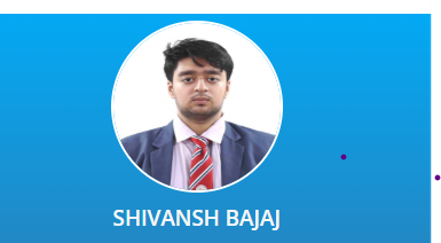
\includegraphics[width=3.0cm,height=1.5cm,keepaspectratio]{member1.png}
\end{minipage}
\\
\hline
\begin{minipage}[t][3.25cm][t]{\linewidth}
\vspace{1.5mm}
\textbf{Team member 2}\\[-1mm]
\textit{(Last Name, name: student ID: email, picture):}
\vspace{2.0cm}
\end{minipage}
&
\begin{minipage}[t][3.25cm][t]{\linewidth}
\vspace{1.5mm}
\textit{Goel, Ashrey -- 2510370302}\\
\textit{2510370302@geu.ac.in}

\vspace{2mm}
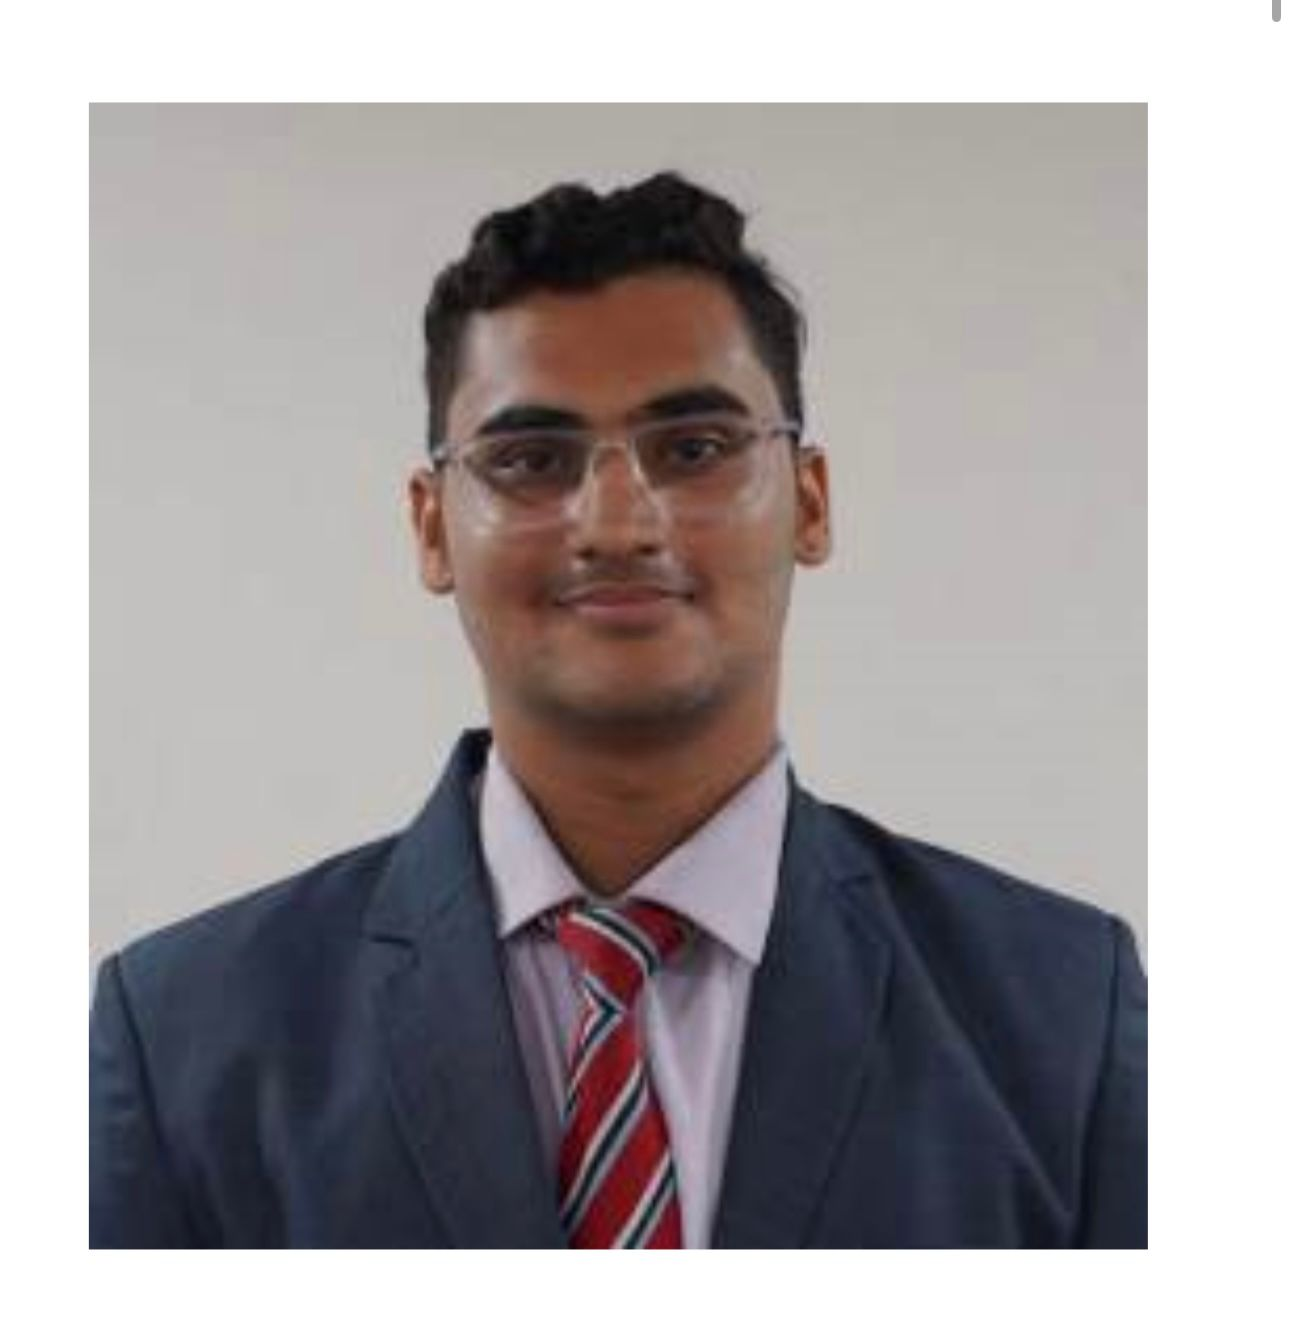
\includegraphics[width=3.0cm,height=1.5cm,keepaspectratio]{member2.png}
\end{minipage}
\\
\hline
\begin{minipage}[t][3.25cm][t]{\linewidth}
\vspace{1.5mm}
\textbf{Team member 3}\\[-1mm]
\textit{(Last Name, name: student ID: email, picture):}
\vspace{2.0cm}
\end{minipage}
&
\begin{minipage}[t][3.25cm][t]{\linewidth}
\vspace{1.5mm}
\textit{Agarwal, Kangana -- 2510380099}\\
\textit{2510380099@geu.ac.in}

\vspace{2mm}
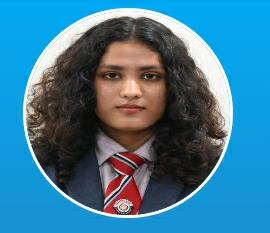
\includegraphics[width=3.0cm,height=1.5cm,keepaspectratio]{member3.png}
\end{minipage}
\\
\hline
\end{tabularx}

\newpage

% -------------------------------------------------
% PAGE 2
% -------------------------------------------------

\bluebigheading{PROPOSAL DESCRIPTION (10 pts)}

\vspace{12mm}

\blueheading{Motivation (1 pt)}

\vspace{1mm}

\answerbox[4.7cm]{\textbf{Problem.} Phishing and social engineering scams are popping up through SMS, email, social media, shady links, phony support messages, and even QR codes—what some are calling 'quishing.' These attackers play on people's sense of urgency, authority, and familiarity with brands to get them to act before double-checking anything. CERT-In has highlighted phishing as a major type of online fraud, mentioning that fake messages often lead users to bogus websites designed to steal their credentials or personal info. A scam can have several red flags: odd wording, strange domains, impersonation, requests for payments, and QR codes. If a detector focuses too narrowly on just one red flag, it might overlook how these signals work together. The Aim of ScamShield is that it treats detection as an \textbf{evidence-fusion problem}: it analyses text, URLs, QR codes and screenshots, combines and mixes those signals and returns an \textbf{interpretable risk score} with the evidence behind the decision.}

\vspace{12mm}

\blueheading{State of the Art / Current solution (1 pt)}

\vspace{1mm


\answerbox[4.5cm]{The current anti-phishing systems use URL blacklists, domain reputation, browser warnings, spam filtering, heuristics and ML classifiers. Sahingoz et al. evaluated seven classifiers using URL and NLP features and reported 36,400 legitimate and 37,175 phishing URLs.
These methods are significantly weaker when malicious content is hidden in an image or QR code. Trad and Chehab proposed direct QR-structure and pixel analysis; their best model achieved an AUC score of 0.9106, improving to 0.9133 after feature refinement. A field study by Sharevski et al. found that convenience strongly influenced the will of users to interact with malicious QR. \textbf{ScamShield extends these directions by combining multiple models and technologies to improve reliability and accuracy and explain the need behind its decision.}}

\vspace{12mm}

\blueheading{Project Goals and Milestones (2 pts)}

\vspace{1mm}


\answerbox[6cm]{
\textbf{Goals:}
\begin{enumerate}
    \item To Detect phishing, smishing, malicious URLs, quishing, and impersonation scams using evidence from text, URLs, screenshots, and QR codes.
    
    \item To Implement the core threat-analysis engine in \textbf{C++ using OOP and DSA}, with an updateable threat knowledge base.
    
    \item To Evaluate the system using \textbf{accuracy, precision, recall, F1-score, false positives, and true positives}.
\end{enumerate}

\textbf{Milestones:} Data collection and preprocessing $\rightarrow$ text and URL analysis $\rightarrow$ QR/OCR analysis $\rightarrow$ C++ OOP/DSA engine $\rightarrow$ evidence fusion and explainability $\rightarrow$ interface integration $\rightarrow$ testing and evaluation.
}


\vspace{3cm}

\blueheading{Project Approach (3 pts)}

\vspace{1mm}


\answerbox[5.7cm]{ScamShield will follow a modular pipeline. Text is analysed for urgency, impersonation, credential requests, suspicious payment language and contextual indicators. URLs are decomposed into structural features such as length, subdomains, special characters and suspicious terms. QR images are decoded where appropriate and can also contribute structural visual signals. Screenshots pass through OCR so visible text and URLs enter the same pipeline.

Each detector produces features and confidence values. A multimodal evidence-fusion layer combines them with threat-intelligence and historical indicators. The core engine is implemented in \textbf{C++}: classes represent inputs, detectors, indicators, evidence and decisions, while vectors, hash tables, stacks, queues and priority queues support storage and analysis.

\textbf{Stack:} C++ for OOP/DSA, Python for data preparation and ML experiments, OpenCV/QR tools and OCR for image processing, standard ML/NLP libraries, and a lightweight web or desktop interface.}

\vspace{1cm}

\blueheading{System Architecture (High Level Diagram)(2 pts)}

\begin{figure}[htbp]
    \centering
    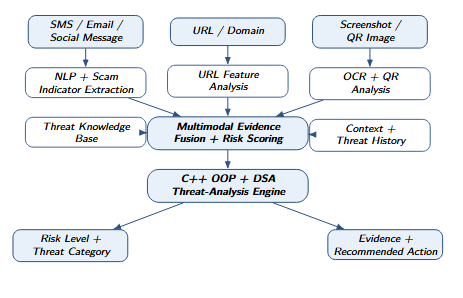
\includegraphics[width=0.7\textwidth]{filename.png}
    \caption{System Architecture Overview}
\end{figure}

\vspace{4mm}
\answerbox[1.75cm]{\textbf{Flow:} Input collection $\rightarrow$ modality-specific extraction $\rightarrow$ threat-intelligence and context aggregation $\rightarrow$ multimodal fusion $\rightarrow$ C++ OOP/DSA threat analysis $\rightarrow$ risk score, evidence and recommended action. The modular design allows individual detectors to be improved without redesigning the full system.}

\vspace{12mm}

\blueheading{Project Outcome / Deliverables (1 pts)}

\vspace{1mm}

\answerbox[2.8cm]{A functional ScamShield prototype containing: (1) a C++ OOP/DSA threat-analysis engine; (2) text, URL, QR and screenshot-analysis modules; (3) an updateable threat knowledge base; (4) multimodal evidence fusion and risk scoring; (5) explainable decision output; (6) a user-facing submission interface; and (7) an evaluation report covering precision, recall, F1-score, false positives and robustness. Source code, data-preparation workflow, architecture documentation and final technical report will accompany the prototype.}

\vspace{6cm}

\blueheading{Assumptions}

\vspace{6mm}

\answerbox[2.65cm]{The submitted text, URLs and images are assumed to be readable. OCR and QR decoding accuracy may vary with image quality, language and noise. External reputation services may be unavailable, so the design cannot depend entirely on blacklists. ScamShield is an \textbf{early-warning and decision-support system}, not a guarantee of safety. Performance depends on representative, current data, and new scam patterns may require knowledge-base or model updates.}

\vspace{12mm}

\blueheading{References}

\vspace{1mm}

\answerbox[5cm]{\scriptsize
\begin{enumerate}[leftmargin=5mm,itemsep=1.8pt,topsep=1pt]
\item Indian Computer Emergency Response Team (CERT-In), ``Preventing Online Scams,'' Advisory CIAD-2024-0050, 24 Oct. 2024. Phishing section: prevalence, impersonation, urgency and counterfeit websites. \href{https://www.cert-in.org.in/}{cert-in.org.in}
\item O. K. Sahingoz, E. Buber, O. Demir and B. Diri, ``Machine learning based phishing detection from URLs,'' \textit{Expert Systems with Applications}, vol. 117, pp. 345--357, 2019. \textbf{Problem context: pp.~345--346.} DOI: 10.1016/j.eswa.2018.09.029.
\item F. Trad and A. Chehab, ``Detecting Quishing Attacks with Machine Learning Techniques Through QR Code Analysis,'' arXiv:2505.03451, 2025. Direct QR-structure analysis for quishing detection. \href{https://arxiv.org/abs/2505.03451}{arxiv.org/abs/2505.03451}
\item F. Sharevski, A. Devine, E. Pieroni and P. Jachim, ``Gone Quishing: A Field Study of Phishing with Malicious QR Codes,'' arXiv:2204.04086, 2022. \href{https://arxiv.org/abs/2204.04086}{arxiv.org/abs/2204.04086}
\item Anti-Phishing Working Group, ``Phishing Activity Trends Report, 1st Quarter 2026,'' 2026. \textbf{Threat summary: pp.~3--4; social-media threats: pp.~6--8.} \href{https://apwg.org/trendreports}{apwg.org/trendreports}
\end{enumerate}
}

\end{document}